\chapter{Implementation}
\label{sec:implementation-chapter}

This chapter introduces the implementation of the proposed
branch-and-cut algorithm which relies on the
latest \textit{CPLEX 22.1 C callable library} (released in March 2022).
The proposed branch-and-cut framework optimally solves the CPTP,
see previous introduction of this problem in \cref{sec:the-capacitated-profitable-tour-problem}.
Our framework can be used as a pricer
inside column generation approaches applied to the standard CVRP,
by appropriately defining the profit function associated to each vertex $p_i \quad \forall i \in V$.
The algorithm's source code is developed in the \textit{C} language,
and it is freely available under a permissive \textit{MIT} license
at the following Github repository: \url{https://github.com/dparo/master-thesis}.

\medskip

\urlref{https://www.ibm.com/analytics/cplex-optimizer}{IBM ILOG CPLEX Optimizer},
CPLEX for short,
is a commercial optimization software package for solving problems expressed as either:
linear programs, mixed-integer programs, quadratic programs, or quadratic constrained programs.
For an introduction to CPLEX refer to \cref{sec:introduction-to-cplex}.

Our branch-and-cut implementation heavily relies on the CPLEX optimizer
to solve the associated MIP model.
The cutting-planes separation was implemented using the \textit{CPLEX generic callback functions},
which have the benefit of not disabling the \textit{Dynamic Search} algorithm,
i.e. the proprietary advanced branch-and-cut algorithm employed internally inside CPLEX,
see discussion in \cref{sec:introduction-to-cplex}.

Compared to tailored pricer algorithms, such as the labeling algorithm \parencite{desrochers1992, feillet2004},
it is clear that using a modern MIP solver, such as CPLEX,
may provide at least two benefits:
(i) parallelization and efficient use of the machine's multiple cores basically for free,
(ii) take advantage of all the engineering effort that went in creating an efficient MIP solver.
However, such an approach also has associated downsides.
Complicated relaxations or constraints,
such as the ng-sets \parencite{baldacci2011},
may be impractical to implement efficiently within a MIP optimizer.

\medskip

We quickly summarize the outline of this chapter.
\Cref{sec:impl-full-static-model} presents the implemented static IP model.
\Cref{sec:impl-warm-starting} describes the implemented primal heuristics
that were used to warm start the CPLEX optimizer.
\Cref{sec:impl-branching} discusses the implemented branching scheme.
Finally, \cref{sec:impl-separation-techniques} describes the implemented cutting-planes strategies,
including a discussion on the employed separation techniques.

\section{Full static model}
\label{sec:impl-full-static-model}

Our static IP model is based on a slight variation of the CPTP formulation
\labelcref{eq:cptp-obj-function,eq:cptp-depot-part-of-tour-constraint,eq:cptp-resource-upper-bound-constraint,eq:cptp-flow-conservation-constraint,eq:cptp-gsec-constraints,eq:cptp-x-mip-var-bounds,eq:cptp-y-mip-var-bounds}
by disregarding the GSECs inequalities \labelcref{eq:cptp-gsec-constraints}.
To guarantee the correctness of the approach,
the GSECs will be exactly separated, during the running-time of the algorithm,
when violation occurs.

We've implemented the following static Integer Programme (IP) model:
\begin{align}
	\min_{x,y} \quad z_\mt{CPTP}(x, y) & = \ExprCptpObjValDef                     & \label{eq:cptp-static-model-0}                         \\
	                                   & y_0 = 1                                  & \label{eq:cptp-static-model-1}                         \\
	                                   & B \le   \ExprCptpDemandSum   \le Q       & \label{eq:cptp-static-model-2}                         \\
	                                   & \ExprCptpEdgesIncident{i}    = 2 y_i     & \quad \forall i \in V  \label{eq:cptp-static-model-3}  \\
	                                   & x_{e}                   \in \Set*{0, 1}  & \quad \forall e \in E  \label{eq:cptp-static-model-4}  \\
	                                   & y_{i}                    \in \Set*{0, 1} & \quad \forall i \in V  \label{eq:cptp-static-model-5},
\end{align}
where
$B \in R_+$ is an additional lower bound on the resource consumption
that may help in gaining a slight improvement on the linear relaxation.
The value of $B$ is computed as $B = q_u + q_v$, where $u, v \in V_0,\ u \ne v$
represent the least two demanding customers in the network:
$q_u \le q_v \le q_i \quad \forall i \in V_0, i \ne u, v$.

\subsection{Upper cutoff value}
\label{sec:impl-upper-cutoff-value}

In the context of pricing for the CVRP,
we're only interested in routes achieving a strictly negative cost function.
The upper cutoff value can help a MIP optimizer
in reducing the number of evaluated branch-and-bound nodes.
The upper cutoff value behaves as a constraint specified directly on the objective function:
\begin{equation}
	z_\mt{CPTP}(x, y) \le 0 - \varepsilon_{\mt{ct}},
\end{equation}
where $\varepsilon_{\mt{ct}} \in \R_+$ is the upper cutoff tolerance.
Most MIP solvers, including CPLEX, has internal support for specifying cutoff values.
However, it is important to note that specifying the cutoff value is not identical
to specifying an explicit constraint in the static model.
Cutoff values contribute only when the branch-and-bound procedure is invoked.
Whereas, an explicit constraint contributes even at the linear relaxation level.
The upper cutoff tolerance $\varepsilon_{\mt{ct}}$ biases the threshold at which the produced
route can be considered a valid reduced cost column.
A non-zero value for $\varepsilon_{\mt{ct}}$ avoids numerical
stability problems caused by the usage of floating point arithmetic
employed in BPC implementations.
To guarantee correctness, the value of $\varepsilon_{\mt{ct}}$ should match the
value employed by the BPC algorithm.
In our case we picked $\varepsilon_{\mt{ct}} = 10^{-6}$,
since it is the value used by the modern BPC framework presented in \textcite{sadykov2021}.

\section{Warm Starting}
\label{sec:impl-warm-starting}

\textit{Warm starting} is a technique which consists in feeding
a MIP optimizer with (good) feasible solutions
prior to starting the resolution process.
Having a set of (good) initial feasible solutions
can tremendously reduce the primal-dual bound gap,
and thus,
decrease amount of time required to reach optimality,
Warm starting can be applied to many IP problem domains,
and it is usually supported by the majors MIP solvers in the market,
such as CPLEX.

Primal heuristic algorithms provide a fast and sensible approach for warm starting.
A CPTP problem has many similarities with TSP.
Therefore,
TSP's heuristics can be readjusted to work successfully even for the CPTP.
Much work was dedicated in studying good heuristics for the TSP,
see \cite{rosenkrantz1977, johnson1997, laporte1992, johnson2007, hoffman2013}.

\medskip

In the remainder of this section,
we explain the warm starting procedure that we've implemented.
The procedure is characterized by two stages:
a constructive insertion heuristic stage (see \cref{sec:impl-insertion-heuristic})
followed by a 2-OPT refinement stage (see \cref{sec:impl-2opt-refinement}),

\subsection{Insertion heuristic}
\label{sec:impl-insertion-heuristic}

\cite{rosenkrantz1977} do a fantastic job in describing the insertion heuristic algorithm
for the TSP and various facets in which it can be implemented.
The insertion heuristic algorithm
can construct a new feasible primal solution in $\Theta(N^2)$ time.
In this section,
we will readjust the TSP insertion heuristic
so that it can be applied to the CPTP.

\medskip

Start by selecting two distinct nodes $u, v \in V,\ q_u + q_v \le Q$
to form an initial tour back-to-back $p = \Tuple*{u, v}$.

The insertion heuristic is an iterative approach,
where at each iteration
an almost-feasible CPTP tour is available.
If the CPTP admits feasible solutions,
when all the iterations of the insertion heuristic are exhausted,
the final available tour will surely be CPTP feasible.
Let's define $q(p) \le Q$ as the total demand served
in by the partial route in the current iteration.
At each iteration,
choose a vertex $a \in p$ and a vertex $h \notin p$.
Let's define $b$ as the successor of node $a$ in the current tour.
The idea is to try to insert $h$ in the tour,
by deleting edge $\Tuple*{a, b}$
and inserting edges $\Tuple*{a, h},\ \Tuple*{h, b}$.
The insertion operation should be performed only
if the $h$ insertion is mandatory to restore feasibility,
or alternatively if it's insertion lowers the route cost.
More formally, let's define the extra mileage as:
\begin{equation}
	\Delta_m(h, a) =
	\begin{cases}
		c_{ah} + c_{hb} - c_{ab} - p_h, & \texttt{if } q(p) + q_h \le Q \\
		\infty,                         & \texttt{otherwise},
	\end{cases}
\end{equation}
which represents the delta route cost in inserting $h$ as the successor of node $a$.
A vertex $h \in V$ is a good candidate for insertion
if at least one of the following conditions is true:
\begin{enumerate}
	\item $\Delta_m(h, a) < 0$, i.e. inserting $h$ improves over the current route.
	\item $h = 0$, i.e. $h$ is the depot node.
	      The depot node at some point must be inserted regardless whether it is improving or not.
	      Note that by convention we have defined $q_0 = 0$,
	      therefore $q(p) + q_0 \le Q$ is always satisfied for the depot node.
	\item The number of visited nodes in the current tour is $2$ and $q(p) + q_h \le Q$.
\end{enumerate}

Prior to insertion the partial route has the form $p = \Tuple*{\dots, a, b, \dots}$;
whereas after the insertion operation completes: $p = \Tuple*{\dots, a, h, b, \dots}$.
In our implementation we employed the \textit{cheapest insertion scheme},
i.e. the pair $(h, a)$ is picked such that it minimizes the extra mileage $\Delta_m(h, a)$
across all possible choices for $a \in p,\ h \notin p$.
The iteration stops when no more valid $h$ vertices can be found for insertion.
At the end of the insertion heuristic, $p$ is a valid route which visits the depot node.
Note that the depot node may not necessarily be the first element of the tour: $p_0 \ne 0$.
A simple circular rotation is sufficient to restore the condition $p_0 = 0$.
It may happen that no valid $h$ can be found,
yet the current tour length is $2$.
In this very unlikely scenario,
we can conclude that the CPTP formulation does not admit any feasible solution
before even solving the IP formulation.

In our implementation we picked $u = 0$ and $v \in V_0$, such that $q_u + q_v \le Q$.
This allows us to generate $O(N)$ good feasible primal solutions using insertion heuristic in $O(N^3)$ time.

\subsection{2-OPT refinement}
\label{sec:impl-2opt-refinement}

Each solution produced from the insertion heuristic
can be further improved using a \textit{2-OPT refinement procedure}.
The 2-OPT algorithm is a heuristic local-search hill-climbing procedure
proposed originally for the TSP in \textcite{flood1956, croes1958} independently.

The 2-OPT algorithm works iteratively requiring $\Omega(N^2)$ number of iterations.
Unfortunately,
as it is pointed out in \textcite{chandra1999},
the 2-OPT procedure may in the worst case take an exponential number of iterations
when fed with purposely artificially constructed instances.
Although this is bad news,
it is also worth pointing out that this rarely occur in practice,
as the probabilistic average number of iterations required for 2-OPT is at most polynomial.

Each iteration of the 2-OPT procedure searches for an existing edge crossing,
and if any exists,
it performs a 2-OPT exchange to undo it.
A 2-OPT exchange is a \textit{primal operation},
i.e. its application preserves route feasibility.
A 2-OPT exchange does not add nor remove vertices from the current route $p$,
therefore the route's gained profit does not change during
the running time of the 2-OPT procedure.
Hence, it is trivial to readjust the original TSP's 2-OPT procedure to the CPTP problem.

Let $a, b \in p$ be two vertices visited in the current route $p$.
Let $a^\prime, b^\prime \in p$ denote respectively the successor of $a$ and $b$ in the current route $p$.
A 2-OPT exchange removes edges $(a, a^\prime)$, $(b, b^\prime)$
in favor of $(a, b)$, $(a^\prime, b^\prime)$
but only if the delta distance, defined as:
\begin{equation}
	\Delta(a, b) = c_{a b} + c_{a^\prime b^\prime} - c_{a a^\prime} - c_{b b^\prime},
\end{equation}
satisfies $\Delta(a, b) < 0$.
If this is the case, performing a 2-OPT exchange over vertices $(a, b)$ lowers the route cost.
After a 2-OPT exchange,
it is necessary to reverse the portion of the route
characterized from the head $a_s$ and tail $b$: $[a_s, \dots, b]$.

In our implementation
we scan for vertices $a, b$ achieving the cheapest exchange,
i.e. for which the delta distance $\Delta(a, b)$ is minimized across all possible valid choices of $a, b \in p$.
The local search algorithms terminates when $\nexists (a, b) \mid a, b \in p,\ \Delta(a, b) < 0$.

\section{Branching}
\label{sec:impl-branching}

\mytodo{Should we enforce strong branching, as is done in @jepsen2014?}

We don't implement any specific branching schemes.
We rely on the branching schemes already provided from the CPLEX MIP optimizer.

\section{Cutting-planes and Inequalities separation}
\label{sec:impl-separation-techniques}

Despite CPLEX already implements internally
the separation of some families of general cutting-planes
(see \cref{sec:introduction-to-cplex}),
generating additional inequalities,
which cannot be deduced from the static model,
can drastically improve the running time of the resolution process.
Cutting-planes separation is a problem which consists
in finding (strong) violated inequalities
so that they can be embedded inside a branch-and-cut framework.
Cutting-planes improve the linear relaxation
by "cutting" fractional points from the convex-hull of integer solutions.
An effective cutting-planes separation strategy
is probably the most important and delicate aspect of any branch-and-cut algorithm \parencite{ralphs2003}.
When evaluating the inclusion of a set of inequalities,
considering the trade-off between the separation cost
and the improvements in the linear relaxation
is a factor of fundamental importance.
Integral inequalities' separation, instead, can be seen as a procedure
to dynamically generate mandatory constraints
that would otherwise be impossible to insert statically into a MIP model.

Additional valid inequalities which are non-strictly necessary to guarantee the algorithm's correctness,
but are computationally expensive to separate exactly,
may be included through a heuristic separation procedure.

Another important factor to take into consideration when implementing
efficient cutting-planes procedures lies in the parametrization settings
of the violated inequalities.
The generation and number of cutting-planes alone (without considering the separation running time),
can highly influence the computation time of the BAC algorithm.
When reporting violated inequalities to the MIP optimizer,
it is usually good practice to define a violation tolerance threshold,
to limit the number of violated inequalities taken into consideration.
Namely, inequalities which are "sufficiently violated" are generated and reported
to the MIP optimizer.
A low violation threshold results in better dual bounds and fewer branch nodes,
but may slower the convergence in each node.
In the opposite way, a high violation threshold results in more branch nodes,
but faster convergence speed \parencite{jepsen2008branchandcut}.

Modern MIP optimizers, such as CPLEX, regardless of the violation threshold
employed in the separation procedure,
can filter each user-provided cuts by scoring them.
Premature branching may occur, regardless of the existence of violated inequalities,
if CPLEX deems these cuts ineffective (tailing off condition).
Scoring cuts costs even more computation time,
for this reason,
it is possible to disable user-cuts filtering.
However, in such case if an effective tailing condition is required,
it must be implemented by the user inside the separation procedure.

\medskip

In our branch-and-cut algorithm,
we are concerned in separating only the
GSECs \labelcref{eq:cptp-gsec-constraints},
RCC \labelcref{eq:cptp-rcc-inequality}
and GLM \labelcref{eq:cptp-glm-inequality}
families of inequalities.
All these inequalities share something in common:
the determination of a subset $S \subseteq V_0$.
A subset $S \subseteq V_0$ can be determined via an appropriate \textit{labeling algorithm},
which determines a partitioning of the network by assigning labels (integer) to each vertex.

The GSECs are the only constraints in our model which must be obligatorily
included through an exact separation procedure.
At a minimum, their inclusion must be devised
for integral solutions of the IP model of
\cref{eq:cptp-static-model-0,eq:cptp-static-model-1,eq:cptp-static-model-2,eq:cptp-static-model-3,eq:cptp-static-model-4,eq:cptp-static-model-5}.
GSEC's can be separated exactly
by tracing the \textit{major connected components}
induced from the integral solution of the model.
Tracing the connected components can be used to determine subsets
$T \subseteq V | \sum_{e \in \delta(T)} x_e = 0$,
which constitutes a valid labeling of the network.
For fractional solutions, however, their exact separation is more complicated.
Let $x^\star \in \R^{|E|}$ denote the value of a fractional solution of
the linear relaxation in
\cref{eq:cptp-static-model-0,eq:cptp-static-model-1,eq:cptp-static-model-2,eq:cptp-static-model-3},
then,
the GSECs can be separated (exactly) by solving $(u, v)$-min-cuts
on a flow neSo che vieni qua, devi fare anche tu le tue cose e non è il posto miglioretwork where capacities are given from the fractional solutions' value $x^\star$.
The $(u, v)$-min-cuts outputs a subset $T \subseteq V$ induced from $(u, v)$
minimizing the term $\sum_{e \in \delta(T)} x^\star_e$,
which constitutes a valid labeling of the network for each $u, v \in V,\ u \ne v$.

Instead, the exact separation of the RCC and GLM inequalities
is a different concern, refer to the respective discussion in \cref{sec:cptp-rcc,sec:cptp-glm}.
For the RCC inequalities,
no exact separation procedure is currently known \parencite{jepsen2014}.
For the GLM inequalities,
a cutting-plane strategy based on solving
$(u, v=0)$-min-cuts on a flow network with $u$-dependent capacities,
may be employed \parencite{letchford2006, jepsen2014}.

\medskip

In our implementation, with regard to the RCC and GLM inequalities,
we opted for a different approach compared to the one proposed in \textcite{jepsen2014}.
We re-use the same integral and fractional labeling algorithms
already employed for the optimal separation of the GSECs inequalities.
These two labeling algorithms will be shared between all the three families of inequalities.
This allows us to limit the programming efforts required to create custom
separation procedure
and also to tremendously reduce the computational impact,
since the same labeling procedures feed the separation of three different families of inequalities.
The labeling algorithms, and the separation procedures of each cuttin-plane,
is implemented in user-provided callbacks using the \textit{CPLEX generic callback API}.

\medskip

In the next two sections, \cref{sec:impl-labeling-integral-solutions,sec:impl-labeling-fractional-solutions},
we will describe the labeling algorithms employed for the integral solutions
and fractional solutions respectively.
Note however, that these two labeling algorithms
are only optimal for the separation of the GSECs inequalities,
while they behave suboptimally (heuristically) for the separation of the RCC and GLM inequalities.
In the remaining sections, instead,
we will discuss the separation of each implemented inequality.

\subsection{Labeling from Integral Solutions}
\label{sec:impl-labeling-integral-solutions}

Our integral labeling algorithm
is devised to be optimal for detecting violated integral GSECs inequalities
of \cref{eq:cptp-static-model-0,eq:cptp-static-model-1,eq:cptp-static-model-2,eq:cptp-static-model-3,eq:cptp-static-model-4,eq:cptp-static-model-5},
but the same procedure is shared
to feed a suboptimal integral separation also for the GLM and RCI inequalities,
as shown in the block diagram in \cref{fig:integral-separation-block-diagram}.

Let $x^\star \in \Set*{0, 1}^{|E|},\ y \in \Set*{0, 1}^{|V|}$ denote the
current integral solution of
\cref{eq:cptp-static-model-0,eq:cptp-static-model-1,eq:cptp-static-model-2,eq:cptp-static-model-3,eq:cptp-static-model-4,eq:cptp-static-model-5}.
If $x^\star, y^\star$ violates a GSEC constraint,
it is easy to verify that the solution models at least a spurious unconnected sub-tour that should be removed.
Unconnected sub-tours can be detected
by computing the \textit{major connected components}
through a Depth-First Search (DFS) traversal
on the network induced from the traversed edges:  $\Set*{e \in E \mid x^\star_e = 1}$.

\medskip

More formally,
let $C = \Set*{-1, 0, \dots, n_c - 1}$ denote the set of connected components
induced from the integral solution $x^\star \in \Set*{0, 1}^{|E|},\ y \in \Set*{0, 1}^{|V|}$.
A vertex $i \in V$ is said to belong to a singleton connected components,
if the connected component contains only $i$ itself, namely $y^\star_i = 0$.
We are only interested in modeling \textbf{major} connected components,
i.e. components containing at least two vertices.
We ignore singleton connected components,
and we associate the sentinel value $-1$ to encode all the vertices $i \in V$ belonging to singletons.
Therefore, the number $n_c \in \Z$ actually represents the number
of major connected components, which satisfies $n_c \ge 1$.
Equivalently,
$n_c$ represents the number of sub-tours formed in the current integral solution.
Let $cc(i) \in C$ be an array
which for each vertex $i \in V$ it encodes to which connected component it belongs to.
Note that the depot node always belongs to a connected component,
therefore by definition we fix $cc(0) = 0$.
For singletons instead we fix $cc(i) = -1  \quad \forall i \in V_0 \mid y^\star_i = 0$.
The connected components can be computed
by a simple DFS traversal, which pseudocode is provided in \cref{algo:cc-dfs}.

Consider the sets $T_k = \Set*{i \in V \mid cc(i) = k}$ with $k = 0, \dots, n_c$
computed from the just devised labeling algorithm.
Due to the construction of such sets,
by letting $k = 0, \dots, n_c$,
it holds that:
$|T_k| \ge 2$,
$\sum_{e \in \delta(T_k)} x^\star_e = 0$
and $\exists i \in T_k \mid y^\star_i = 1$.
Therefore, this approach ensures correctness of the whole branch-and-cut procedure.


\begin{algorithm}
	\caption{An algorithm for computing the major connected components through a Depth-First Search (DFS) traversal}
	\KwData{$x^\star \in \Set*{0, 1}^{|E|},\ y^\star \in \Set*{0, 1}^{|V|}$: current integral solution of
		\cref{eq:cptp-static-model-0,eq:cptp-static-model-1,eq:cptp-static-model-2,eq:cptp-static-model-3,eq:cptp-static-model-4,eq:cptp-static-model-5}
	}
	\KwResult{$n_c$: number of subtours formed}
	\KwResult{$cc[i] \in C$: connected component of $\forall i \in V$}
	\Proc{\textit{cc\_dfs}($x^*$, $y^*$)}{
	\Let $cc[i] \gets -1 \quad \forall i \in V$\;
	\Let $nc \gets 0$\;
	\For{$i\gets0$ \KwTo $N$}{
		\If{$cc[i] < 0, y^*_i = 1$}{
			\Comment{Found a non visited sub-tour}
			$cc[i] \gets n_c$\;
			\Let $u \gets -1$\;
			\Comment{Traverse the sub-tour}
			\Do{$u \ge 0$}{
				\Let $v \gets -1$\;
				\For{$j \in V \mid e = \Set*{u, j} \in E,\ cc[j] < 0,\ x^*_{e} = 1$}{
					\Comment{The body of this loop will execute only once}
					$cc[j] = n_c$\;
					$v \gets j$\;
				}
				$u \gets v$
			}
			$n_c \gets n_c + 1$\;
		}
	}

	\Comment{Validate some invariants}
	\Assert{$n_c \ge 0$}\;
	\Assert{$c[0] = 0$}\;
	\Assert{$c[i] = -1 \quad \forall i \in V_0 \mid y^*_i = 0$}\;
	\Assert{$c[i] \ge 0 \quad \forall i \in V_0 \mid y^*_i = 1$}\;
	\Comment{Done: terminate}
	\Return{$n_c, cc$}
}

	\label{algo:cc-dfs}
\end{algorithm}


\begin{figure}[ht]
	\centering
	\framebox{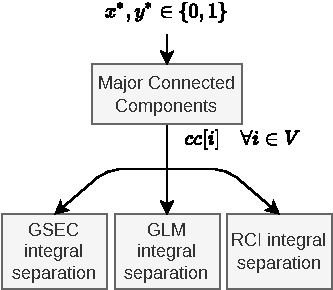
\includegraphics[width=6cm]{Imgs/integral-separation-block-diagram.cropped.pdf}}
	\caption{A block diagram representing the structure
		of the employed separation structure for integral solutions
		along with the shared labeling algorithm.
	}
	\label{fig:integral-separation-block-diagram}
\end{figure}

\subsection{Labeling from Fractional Solutions}
\label{sec:impl-labeling-fractional-solutions}

Our fractional labeling algorithm is devised to be optimal for
detecting violated fractional GSECs inequalities
of \cref{eq:cptp-static-model-0,eq:cptp-static-model-1,eq:cptp-static-model-2,eq:cptp-static-model-3},
but the same procedure is shared
to feed a suboptimal fractional separation also for the GLM and RCI inequalities,
as shown in the block diagram in \cref{fig:fractional-separation-block-diagram}.
This algorithm is inherently more difficult, and computationally expensive,
compared to the integral labeling algorithm.

A valid set $T \subseteq V$ can be separated for a fractional $x^\star \in \R^{|E|},\ y^\star \in \R^{|V|}$,
by solving a
max-flow problem between two arbitrary source and sink vertices $u, v \in V,\ u \ne v$ on a fully connected directed graph.
The max-flow problem is modeled through a directed symmetric flow network,
where the capacities $w_{ij} \in \R \quad \forall i, j \in V$
are given from the current fractional solution $w_{ij} = x^\star_{\Set*{i, j}} \quad \forall i, j \in V$.

A solution to the max-flow problem
outputs a maxflow $\maxflow(u, v)$ and a bipartition, also called "binary coloring",
of the set $V$,
namely two complementary sets $F_1(u, v),\ F_2(u, v)$
such that $F_1(u, v) \cup F_2(u, v) = V$, $F_1 \cap F_2 = \emptyset$ and $u \in F_1(u, v),\ t \in F_2(u, v)$.
The quantity $\delta(F_1(u, v))$ constitutes the min-cut induced from solving the max-flow problem over $(u, v)$.
It is known that solving a maxflow problem guarantees the following two properties:
\begin{enumerate}
	\item Arcs $\{ (i, j) \mid i \in F_1(u, v),\ j \in F_2(u, v) \}$ are saturated
	\item Arcs $\{ (j, i) \mid i \in F_1(u, v),\ j \in F_2(u, v) \}$ are drained.
\end{enumerate}
Therefore the following result holds:
\begin{align}
	\sum_{(i, j) \in \deltaplus(F_1(u, v))} f_{ij}  & = \sum_{(i, j) \in \deltaplus(F_1(u, v))} x^\star_{\Set*{i, j}} & = \maxflow(u, v) \\
	\sum_{(i, j) \in \deltaminus(F_1(u, v))} f_{ij} & = \sum_{(i, j) \in \deltaplus(F_2(u, v))} f_{ij}                & = 0,
\end{align}
where $f_{ij}$ denotes the flow along the directed arcs $(i, j),\ i, j \in V$ in the corresponding flow network.

It is important to note that,
since we are dealing with a \textbf{symmetrical} flow network,
solving the maxflow problem between pairs $(u, v)$ and pair $(u, v)$ will output the same maxflow value,
i.e. $\maxflow(u, v) = \maxflow(v, u)$.
Although, and this is the more important aspect,
the induced bipartitions in the general case are not guaranteed to be symmetric.
Namely, in the general case we have that: $F_1(u, v) \ne F_2(u, v)$ and $F_2(u, v) \ne F_1(u, v)$.
To see this is the case, this simple flow network:
\begin{center}
	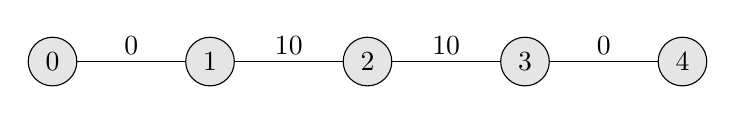
\begin{tikzpicture}[node distance={20mm}, main/.style = {draw, circle, fill=black!10!white}]
		\centering

		\node[main] (0) {$0$};
		\node[main] (1) [right of = 0] {$1$};
		\node[main] (2) [right of = 1] {$2$};
		\node[main] (3) [right of = 2] {$3$};
		\node[main] (4) [right of = 3] {$4$};

		\draw (0) --  (1) node [midway, yshift=2mm] {$0$};
		\draw (1) --  (2) node [midway, yshift=2mm] {$10$};
		\draw (2) --  (3) node [midway, yshift=2mm] {$10$};
		\draw (3) --  (4) node [midway, yshift=2mm] {$0$};
	\end{tikzpicture}
\end{center}
produces the same maxflow value when solving for $(0, 4)$ and $(4, 0)$ pair respectively,
and produces $F_1(0, 4) = \{ 0\},\ F_2(0, 4) = \{ 1, 2, 3, 4\}$, $F_1(4, 0) = \{ 4 \},\ F_2(4, 0) = \{ 0, 1, 2, 3\}$,
which clearly represent a non symmetric coloring.
This behavior is a direct consequence that flow networks don't guarantee unique min-cuts.

\medskip

In this thesis,
we used the push relabel max flow algorithm first developed in \cite{goldberg1997},
which in practice it is usually faster than more classical approaches such as the Ford-Fulkerson max-flow algorithm.
The push relabel max flow algorithm runs in $O(N^4)$ time,
and when combined with an exhaustive enumeration over all possible choices of $u, v \in V,\ u \ne v$,
can take up to $O(N^6)$ time.

The Gomory-Hu tree, first presented in \cite{gomory1961},
provides a way to compute the all pairs $(u, v)$ max-flows using only $N$ main max-flow computations.
A Gomory-Hu tree can be seen as a data structure that represents a simpler reduced flow network,
where max-flow computations become trivially solvable
through a single iteration of the Ford-Fulkerson algorithm in $\Theta(N^2)$.
Combining Gomory-Hu trees and the push relabel max flow algorithm,
an exhaustive enumeration of all possible $(u, v)$ vertices takes up to $O(N^5)$ time to build the tree
and further $\Theta(N^4)$ to query for all the possible $F_1(u, v), F_2(u, v)$ bipartitions.

In our implementation
we exploited the Gomory-Hu tree to provide full enumeration of all possible $(u, v)$ maxflows.
For brevity reasons we will not list the pseudocode of the max-flow and Gomory-Hu tree algorithms.
Refer to the \urlref{https://github.com/dparo/master-thesis}{Github repository} for their respective implementation.

\medskip

We conclude the section by providing an implementation tip.
Writing fast and correct max-flow algorithms that operate directly with floating point arithmetic
can be difficult and error-prone due to accumulation of accuracies errors.
Any trivial implementation may "get stuck" in massively long loops pushing atomically small quantity of flows.
Careful attention must be paid when developing one such algorithm.
Good software engineering practices, such as unit testing, can help in spotting problematic implementations.

A simpler approach consists in implementing a maxflow algorithm that operates with integer arithmetic.
By exploiting that $x^\star$ is bounded in the $[0, 1]$ range,
we can multiply the fractional solution value $x^\star$ by a big-constant $M \in \R$ (e.g. $M = 10^6$)
and truncate its value when defining the capacities of the flow network.
The value $\maxflow(u, v)$ then needs to be remapped on the original scale
by dividing it by $M$.
For simplicity and stability, in our maxflow implementation we opted for the latter approach.


\begin{figure}[ht]
	\centering
	\framebox{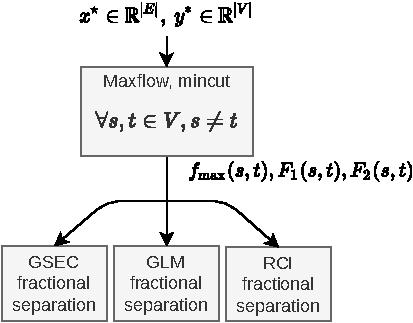
\includegraphics[width=8cm]{Imgs/fractional-separation-block-diagram.cropped.pdf}}
	\caption{A block diagram representing the structure
		of the employed separation structure for fractional solutions
		along with the shared labeling algorithm.
	}
	\label{fig:fractional-separation-block-diagram}
\end{figure}

\begin{comment}
[@dparo: Old Gomoru HU Tree, It was slow and required amortization to speed up the BAC procedure]
Since running this full enumeration over each fractional separation,
turned out to be quite costly, we decided to amortize the cost over multiple iterations.
Namely, fractional separations iterations which are not multiple of $N$ become a no-op,
no max-flow is performed and therefore no set $S \subseteq V_0$ is separated.
\end{comment}

\subsection{GSEC Separation}
\label{sec:impl-gsec-separation}


\subsubsection{GSEC Integral Separation}
\label{sec:impl-gsec-integral-separation}

The GSEC integral separation procedure is the most important
separation procedure in our implementation,
since it is mandatory to ensure the correctness of the branch-and-cut algorithm.
GSECs inequalities which are violated by integral solutions
must be separated exactly and reported as is
(without employing violation thresholds) to the MIP optimizer.

The GSEC requires the separation of a subset $S \subseteq V_0$.
Let $T_k  = \Set*{i \in V \mid cc(i) = k},\ |T_k| \ge 1 \quad \forall k \in \Set*{1, \dots, n_c}$ be the labeling
outputted from the major connected components as discussed in \cref{sec:impl-labeling-integral-solutions}.
By construction $n_c \ge 1,\ 0 \in T_0$.
Then a valid subset $S \subseteq V_0$ can be picked as $S = T_k \quad \forall k \in \Set*{1, \dots, n_c}$.
Which implies that,
any major connected component (i.e. sub-tour) that does not contain the depot node,
can be used as a valid set $S \subseteq V_0$ for separating GSEC inequalities from integral solutions.
If $n_c = 1$ then no $S \subseteq V_0$ can be separated,
which implies that the current integral solution models an optimal solution for the whole CPTP formulation
\labelcref{eq:cptp-obj-function,eq:cptp-depot-part-of-tour-constraint,eq:cptp-resource-upper-bound-constraint,eq:cptp-flow-conservation-constraint,eq:cptp-gsec-constraints,eq:cptp-x-mip-var-bounds,eq:cptp-y-mip-var-bounds}.


Let $x^\star \in \Set*{0, 1}^{|E|},\ y \in \Set*{0, 1}^{|V|}$ denote the
current integral solution of
\cref{eq:cptp-static-model-0,eq:cptp-static-model-1,eq:cptp-static-model-2,eq:cptp-static-model-3,eq:cptp-static-model-4,eq:cptp-static-model-5}.
Recall the GSEC inequality definition in \cref{eq:cptp-gsec-constraints},
it is easy to verify that:
\begin{equation}
	\sum_{e \in \delta(S)} x^*_{e} = 0, \qquad y_i =  1 \quad \forall i \in S
\end{equation}
which implies that \cref{eq:cptp-gsec-constraints} cannot be satisfied by any $i \in S$.

\medskip

In a single integral separation iteration we can therefore separate:
\begin{equation}
	\sum^{n_c}_{k = 1} \SetSize*{ \Set*{ i \mid cc(i) = k \quad \forall i \in V } }
\end{equation}
violated GSECs inequality, which can be promptly reported to the MIP solver to reject the candidate integral solution.

A complete pseudocode of the GSEC integral separation procedure is provided in \cref{algo:gsec-integral-sep}.

\begin{algorithm}
	\caption{An algorithm for separating GSEC integral inequalities for the CPTP}
	\label{algo:gsec-integral-sep}
	\KwResult{$n_c$: number of major connected components}
	\KwData{$cc[i] \in C$: connected component $\forall i \in V$, see \cref{sec:impl-labeling-integral-solutions}}
	\KwData{$x^\star \in \Set*{0, 1}^{|E|},\ y^\star \in \Set*{0, 1}^{|V|}$: current integral solution of
		\cref{eq:cptp-static-model-0,eq:cptp-static-model-1,eq:cptp-static-model-2,eq:cptp-static-model-3,eq:cptp-static-model-4,eq:cptp-static-model-5}
	}
	\Proc{\textit{gsec\_integral\_sep}($n_c$, $cc$, $x^\star$, $y^\star$)}{
	\For{$k \gets 1$ \KwTo $n_c$}{
		\Let $S \gets  \Set* {i \mid cc[i] = k}$\;
		\Assert{$|S| \ge 2$}\;
		\Comment{Build the cut}
		\Let nnz $\gets$ 0, index $\gets$ [], value $\gets$ []\;
		\For{$e = \Set*{i, j} \in E \mid i \in S,\ j \notin S$}{
			index[nnz] $\gets$ x\_mip\_var\_idx($e$)\;
			value[nnz] $\gets$ $1$\;
			nnz $\gets$ nnz + $1$\;
		}
		\For{$i \in S$}{
			index[nnz] $\gets$ y\_mip\_var\_idx($i$)\;
			value[nnz] $\gets$ $-2.0$\;
			\Comment{Reject and report cut to MIP}
			mip\_add\_user\_cut(nnz, index, value)\;
		}
	}
}

\end{algorithm}





\subsubsection{GSEC Fractional Separation}
\label{sec:impl-gsec-fractional-separation}

In our implementation, GSECs separation for integral solutions is always exhaustively applied.
The separation of GSEC inequalities for fractional solutions,
while it is non-strictly required for our implementation,
can dramatically reduce the number of branch nodes if properly applied.

Let $\maxflow(u, v),\ F_1(u, v),\ F_2(u, v)$ denote the maxflow value and bipartitions
produced from the labeling algorithm described in \cref{sec:impl-labeling-fractional-solutions}.
A valid $S \subseteq V_0$ for separating GSEC inequalities from fractional solution can be picked such that:
\begin{equation}
	S \subseteq V_0 =
	\begin{cases}
		F_1(u, v), & \texttt{if } 0 \notin F_1(u, v) \\
		F_2(u, v), & \texttt{otherwise}
	\end{cases},
	\qquad
	|S| \ge 2
\end{equation}
Such approach can feed up to
$N^2 - N$ different sets $S \subseteq V_0$,
one for each possible pair $\Tuple*{u, v} \in V^2,\ u \ne v$


Let $x^\star \in \R^{|E|},\ y \in \R^{|V|}$ denote the
current fractional solution of
\cref{eq:cptp-static-model-0,eq:cptp-static-model-1,eq:cptp-static-model-2,eq:cptp-static-model-3}.
Recall the GSEC inequality definition in \cref{eq:cptp-gsec-constraints},
it is easy to verify that $\sum_{e \in \delta(S)} x^*_{ij} = \maxflow(u, v)$
due to the symmetry property of the flow network.

Therefore, any $i \in S$ that violates $\maxflow(s, t) \ge 2 y_i$
can be used to separate a violated GSEC inequality.
With such approach t is possible to separate $O(N^3)$ GSECs per fractional solution.
We noticed that, generating and reporting all this violated GSECs inequalities
led to a slow-down of the MIP optimizer.

\medskip
In our implementation we opted for a different approach by relaxing the conditions at which these cuts are reported.
For each subset $S \subseteq V_0,\ |S| \ge 2$, we report only the single most violated GSEC
associated to the customer $i \in V_0$ that maximizes the $\maxflow(u, v) - 2 y_i$ violation.
On top of that, to limit the number of weak GSEC inequalities that are reported to the MIP optimizer,
we define a violation threshold $\varepsilon_{\mt{GSEC}}$ and report the associated cut only if:
\begin{equation}
	\maxflow(s, t) \ge 2 y_i - \varepsilon_{\mt{GSEC}}
\end{equation}
is violated.
In our implementation we picked $\varepsilon_{\mt{GSEC}} = \epsGsecFValue$.

A complete pseudocode of the GSEC fractional separation procedure is provided in \cref{algo:gsec-frac-sep}.

\begin{algorithm}
	\caption{An algorithm for separating GSEC fractional inequalities for the CPTP}
	\label{algo:gsec-frac-sep}
	\KwData{$\maxflow(s, t), F_1(s, t), F_2(s, t)$: maxflow and bipartitions induced from an arbitrary $s \ne t, s \in V, t \in V$ pair}
	\KwData{$x^\star \in \R^{|E|},\ y^\star \in \R^{|V|}$: current fractional solution of
		\cref{eq:cptp-static-model-0,eq:cptp-static-model-1,eq:cptp-static-model-2,eq:cptp-static-model-3}
	}
	\Proc{\textit{gsec\_frac\_sep}($\maxflow(u, v)$, $F_1(u, v)$, $F_2(u, v)$, $x^\star$, $y^\star$)}{
	\Const sense $\gets$ '$\ge$'\;
	\Const rhs $\gets$ $0$\;
	\Const $\varepsilon_{\mt{GSEC}} \gets \epsGsecFValue$\;

	\Let $S$\;
	\uIf{$0 \notin F_1(u, v)$}{
		$S \gets F_1(u, v)$\;
	}\Else{
		$S \gets F_2(u, v)$\;
	}

	\Comment{Scan for most violated customer}
	\Let $c \gets -1$, $m \gets \infty$\;
	\For{$i \in V \mid i \in S$}{
		\Let $v \gets \maxflow(u, v) - 2 y^*_i$\;

		\If{$\Expr*{\maxflow(u, v) < 2 y^*_i - \varepsilon_{\mt{GSEC}}}$ \And $v < m$}{
			$c \gets i$\;
			$m \gets v$\;
		}
	}

	\If{$c \ge 0$ \And $|S| \ge 2$}{
		\Comment{Build the cut}
		\Let nnz $\gets$ 0, index $\gets$ [], value $\gets$ []\;
		\For{$e = \Set*{i, j} \in E \mid i \in S,\ j \notin S$}{
			index[nnz] $\gets$ x\_mip\_var\_idx($e$)\;
			value[nnz] $\gets$ $1.0$\;
			nnz $\gets$ nnz + $1$\;
		}

		index[nnz] $\gets$ y\_mip\_var\_idx($c$)\;
		value[nnz] $\gets$ $-2.0$\;
		nnz $\gets$ nnz + $1$\;
		\Comment{Reject and report cut to MIP}
		mip\_add\_user\_cut(sense, rhs, nnz, index, value)\;
	}
}

\end{algorithm}

\subsection{RCC separation}
\label{sec:impl-rcc-separation}

In this section we describe the separation of the RCC inequalities, as they were defined in Equation \eqref{eq:cptp-rcc-inequality}.
In our work we implemented both the integral and the fractional separation for this family of inequalities.
However, we will omit the detail of the integral separation in this section, since they follow naturally from ideas explained in previous sections.

The fractional separation of RCC inequalities is not any different from the separation of the GLM fractional inequalities presented in \cref{sec:glm-separation}.
The only difference is that the set $S \subseteq V_0$, does not need to satisfy $\SetSize*{S} \ge 2$.

Therefore, a set $\SetSize*{S} \subseteq V_0$ can separate a single RCC cut if the following inequality

\begin{equation}
	\begin{split}
		\ExprCptpFlowExiting{S} -2 \ExprCptpServedDemandWithWeight{S}{i}{\frac{q_i}{\ExprQr(S)}}    \ge   2 \left( \ceil*{ \frac{q(S)}{Q}} - \frac{q(S)}{Q_{\mathrm{R}}(S)} \right) - \varepsilon_{\mt{RCC}}
	\end{split}
\end{equation}

is violated.
The $\varepsilon_{\mt{RCC}}$ is a constant which denotes the violation tolerance for the RCC fractional separation.
In our implementation we picked $\varepsilon_{\mt{RCC}} = \epsRccFValue$.
We can separate $O(N^2)$ RCC cuts since the number of set $S \subseteq V_0$ is in the order of $\Theta(N^2)$ per fractional separation iteration.

The complete pseudocode for both the integral and fractional separation can be found in \cref{algo:rcc-integral-sep,algo:rcc-frac-sep} respectively.

\begin{algorithm}
	\caption{An algorithm for separating RCC integral inequalities for the CPTP}
	\label{algo:rcc-integral-sep}
	\KwResult{$n_c$: number of subtours formed}
	\KwData{$cc[i] \in C$: connected component of $\forall i \in V$}
	\KwData{$x^*, y^* \in \{0, 1\}$: current integral solution of
		\cref{eq:cptp-static-model-0,eq:cptp-static-model-1,eq:cptp-static-model-2,eq:cptp-static-model-3,eq:cptp-static-model-4,eq:cptp-static-model-5}
	}
	\Proc{\textit{rcc\_integral\_sep}($n_c$, $cc$, $x^\star$, $y^\star$)}{
	\Const sense $\gets$ '$\ge$'\;

	\For{$k \gets 1$ \KwTo $n_c$}{
		\Const $S \gets  \Set* {i \mid cc[i] = k}$\;
		\Const $Q_S$ $\gets \sum\limits_{i \in S} q_i$\;
		\Const $Q_R$ $\gets$ $\mod(Q_S, Q)$\;
		\Const rhs $\gets$ $2 \Expr*{\ceil*{\frac{Q_S}{Q}} - \frac{Q_S}{Q_R}}$\;

		\If{$Q_R > 0$ \And $|S| \ge 1$}{
			\If{$-2 \sum\limits_{i \in S} \frac{q_i}{Q_R} y^*_i  < $ rhs}{
				\Comment{Build the cut}
				\Let nnz $\gets$ 0, index $\gets$ [], value $\gets$ []\;
				\For{$e = \Set*{i, j} \in E \mid i \in S,\ j \notin S$}{
					index[nnz] $\gets$ x\_mip\_var\_idx($e$)\;
					value[nnz] $\gets$ $1$\;
					nnz $\gets$ nnz + $1$\;
				}
				\For{$i \in S$}{
					index[nnz] $\gets$ y\_mip\_var\_idx($i$)\;
					value[nnz] $\gets$ $-2 q_i / Q_R$\;
					nnz $\gets$ nnz + $1$\;
				}
				\Comment{Reject and report cut to MIP}
				mip\_add\_user\_cut(sense, rhs, nnz, index, value)\;
			}
		}
	}
}

\end{algorithm}

\begin{algorithm}
	\caption{An algorithm for separating RCC fractional inequalities for the CPTP}
	\label{algo:rcc-frac-sep}
	\KwData{$\maxflow(s, t), F_1(s, t), F_2(s, t)$: maxflow and bipartitions induced from an arbitrary $s \ne t, s \in V, t \in V$ pair}
	\KwData{$x^\star \in \R^{|E|},\ y^\star \in \R^{|V|}$: current fractional solution of
		\cref{eq:cptp-static-model-0,eq:cptp-static-model-1,eq:cptp-static-model-2,eq:cptp-static-model-3}
	}
	\Proc{\textit{rcc\_frac\_sep}($n_c$, $cc$, $x^*$, $y^*$)}{
	\Const $\varepsilon_{\mt{RCI}} \gets \epsRccFValue$\;

	\For{$c \gets 1$ \KwTo $n_c$}{
		\Let $S$\;
		\uIf{$0 \notin F_1(s, t)$}{
			$S \gets F_1(s, t)$\;
		}\Else{
			$S \gets F_2(s, t)$\;
		}
		\Let $Q_S$ $\gets \sum_{i \in S} q_i$\;
		\Let $S_S$ $\gets \sum_{i \in S} y^*_i \cdot q_i$\;
		\Let $Q_R$ $\gets$ $\mod(Q_S, Q)$\;
		\If{$Q_R > 0$ \And $|S| \ge 1$}{
			\If{$\maxflow(s, t) -2 S_S / Q_R$ $<$ $2 \ceil*{Q_S / Q} - 2 Q_S / Q_R$ - $\varepsilon_{\mt{RCI}}$}{
				\Comment{Build the cut}
				\Let nnz $\gets$ 0, index $\gets$ [], value $\gets$ []\;
				\For{$i \in V \mid i \in S$}{
					index[nnz] $\gets$ y\_mip\_var\_idx($i$)\;
					value[nnz] $\gets$ $-2 q_i / Q_R$\;
					nnz $\gets$ nnz + $1$\;

					\For{$j \in V \mid j \notin S$}{
						index[nnz] $\gets$ x\_mip\_var\_idx($i$, $j$)\;
						value[nnz] $\gets$ $1$\;
						nnz $\gets$ nnz + $1$\;
					}
				}
				\Comment{Reject and report cut to MIP}
				mip\_add\_user\_cut(nnz, index, value)\;
			}
		}
	}
}

\end{algorithm}

\subsection{GLM separation}
\label{sec:impl-glm-separation}

In this section we describe the separation of the GLM inequalities, as they were defined in Equation \eqref{eq:glm-inequality}.
In our work we implemented both the integral and the fractional separation for this family of inequalities.
However, in this section we will explain only the fractional separation and we will omit the details about integral separation.
The integral separation follows naturally from adapting the ideas that will here after be presented in this section, and by employing a similar reasoning as was done in \cref{sec:gsec-integral-separation}, for the GSEC inequalities (i.e. using the connected components).

Let $F_1(s, t),\ F_2(s, t)$ be the bipartition induced in solving the min-cut problem as was presented in \cref{sec:fractional-separation}.
Again we showed that we can pick a valid $S \subseteq V_0$ in the following way

\begin{equation}
	S \subseteq V_0 =
	\begin{cases}
		F_1(s, t), & \texttt{if } 0 \notin F_1 \\
		F_2(s, t), & \texttt{otherwise}
	\end{cases}
\end{equation}

In case of the integral separation the same reasoning apply here, but instead of using the min-cut bipartition, we use the connected components array to find a valid $S \subseteq V_0$.

We need to count the number of vertices $i$ in $S$ to verify that indeed $\SetSize*{S} \ge 2$.
If $\SetSize*{S} < 2$, no GLM inequalities can be separated.
Otherwise a single GLM cut can be separated if the following inequality

\begin{equation}
	\begin{split}
		\ExprCptpFlowExitingWithWeight{S}{\Expr*{1 - 2 \frac{q_j}{Q}}} - 2 	\ExprCptpServedDemandWithWeight{S}{i}{\frac{q_i}{Q}} \ge - \varepsilon_{\mt{GLM}}
	\end{split}
\end{equation}

is violated.
The $\varepsilon_{\mt{GLM}}$ is a constant which denotes the violation tolerance for the GLM fractional separation.
In our implementation we picked $\varepsilon_{\mt{GLM}} = \epsGlmFValue$.
We can separate $O(N^2)$ GLM cuts since the number of set $S \subseteq V_0$ is in the order of $\Theta(N^2)$ per fractional separation iteration.

The complete pseudocode for both the integral and fractional separation can be found in \cref{algo:glm-integral-sep, algo:glm-frac-sep} respectively.

\begin{algorithm}
	\caption{An algorithm for separating GLM integral inequalities for the CPTP}
	\label{algo:glm-integral-sep}
	\KwResult{$n_c$: number of subtours formed}
	\KwData{$cc[i] \in C$: connected component of $\forall i \in V$}
	\KwData{$x^*, y^* \in \{0, 1\}$: current integral solution of
		\cref{eq:cptp-static-model-0,eq:cptp-static-model-1,eq:cptp-static-model-2,eq:cptp-static-model-3,eq:cptp-static-model-4,eq:cptp-static-model-5}
	}
	\Proc{\textit{glm\_integral\_sep}($n_c$, $cc$, $x^*$, $y^*$)}{
	\Const $\varepsilon_{\mt{GLM}} \gets 0.01$\;

	\For{$c \gets 1$ \KwTo $n_c$}{
		\Let $S \gets  \Set* {i \mid cc[i] = c}$\;
		\If{$|S| \ge 2$}{
			\Comment{Build the cut}
			\Let lhs $\gets 0$\;
			\Let nnz $\gets$ 0, index $\gets$ [], value $\gets$ []\;
			\For{$i \in V \mid i \in S$}{
				\For{$j \in V \mid j \notin S$}{
					index[nnz] $\gets$ x\_mip\_var\_idx($i$, $j$)\;
					value[nnz] $\gets$ $1 - 2 q_j / Q$\;
					lhs $\gets$ lhs + $x^*_{ij} \cdot (1 - 2 q_j / Q)$\;
					nnz $\gets$ nnz + $1$\;
				}
			}
			\For{$i \in V \mid i \in S$}{
				index[nnz] $\gets$ y\_mip\_var\_idx($i$)\;
				value[nnz] $\gets$ $-2 q_i / Q$\;
				lhs $\gets$ lhs + $y^*_{i} \cdot (2 q_i / Q)$\;
				nnz $\gets$ nnz + $1$\;
			}
			\If{\Not lhs $\ge$ $-\varepsilon_{\mt{GLM}}$}{
				\Comment{Reject and report cut to MIP}
				mip\_add\_user\_cut(nnz, index, value)\;
			}
		}
	}
}

\end{algorithm}

\begin{algorithm}
	\caption{An algorithm for separating GLM fractional inequalities for the CPTP}
	\label{algo:glm-frac-sep}
	\KwData{$\maxflow(s, t), F_1(s, t), F_2(s, t)$: maxflow and bipartitions induced from an arbitrary $s \ne t, s \in V, t \in V$ pair}
	\KwData{$x^\star \in \R^{|E|},\ y^\star \in \R^{|V|}$: current fractional solution of
		\cref{eq:cptp-static-model-0,eq:cptp-static-model-1,eq:cptp-static-model-2,eq:cptp-static-model-3}
	}
	\Proc{\textit{glm\_frac\_sep}($\maxflow(u, v)$, $F_1(u, v)$, $F_2(u, v)$, $x^\star$, $y^\star$)}{
	\Const sense $\gets$ '$\ge$'\;
	\Const rhs $\gets$ $0$\;
	\Const $\varepsilon_{\mt{GLM}} \gets \epsGlmFValue$\;
	\Let $S$\;
	\uIf{$0 \notin F_1(u, v)$}{
		$S \gets F_1(u, v)$\;
	}\Else{
		$S \gets F_2(u, v)$\;
	}

	\If{$|S| \ge 2$}{
		\Comment{Build the cut}
		\Let lhs $\gets 0$\;
		\Let nnz $\gets$ 0, index $\gets$ [], value $\gets$ []\;
		\For{$i \in V \mid i \in S$}{
			\For{$j \in V \mid j \notin S$}{
				index[nnz] $\gets$ x\_mip\_var\_idx($i$, $j$)\;
				value[nnz] $\gets$ $1 - 2 q_j / Q$\;
				lhs $\gets$ lhs + $x^\star_{ij} \cdot (1 - 2 q_j / Q)$\;
				nnz $\gets$ nnz + $1$\;
			}
		}
		\For{$i \in V \mid i \in S$}{
			index[nnz] $\gets$ y\_mip\_var\_idx($i$)\;
			value[nnz] $\gets$ $-2 q_i / Q$\;
			lhs $\gets$ lhs + $y^*_{i} \cdot (2 q_i / Q)$\;
			nnz $\gets$ nnz + $1$\;
		}
		\If{\Not lhs $\ge$ $-\varepsilon_{\mt{GLM}}$}{
			\Comment{Reject and report cut to MIP}
			mip\_add\_user\_cut(sense, rhs, nnz, index, value)\;
		}
	}
}

\end{algorithm}
